\documentclass[11pt,a4paper]{article}
\usepackage[T1]{fontenc}
\usepackage[utf8]{inputenc}
\usepackage{lmodern,microtype}
\usepackage[margin=.85in]{geometry}
\usepackage{amsmath,amssymb,mathtools}
\usepackage{booktabs,tabularx,array,enumitem,needspace,float}
\usepackage{xcolor,tikz}
\usetikzlibrary{arrows.meta,positioning,fit,calc,backgrounds}
\usepackage[hidelinks]{hyperref}
\usepackage[nameinlink,noabbrev]{cleveref}
\usepackage{fancyhdr}
\hypersetup{pdftitle={Sequencer Rotation Architecture v2},
pdfsubject={Module interfaces, unified publication verification, and staking lifecycle}}
\pagestyle{fancy}\fancyhf{}
\lhead{\small Sequencer rotation architecture}\rhead{\small Version 2 / Part II baseline}
\cfoot{\thepage}\setlength{\headheight}{14pt}
\setlength{\parindent}{0pt}\setlength{\parskip}{4pt}
\setlength{\emergencystretch}{2em}
\setlist{nosep,leftmargin=*}
\newcolumntype{Y}{>{\raggedright\arraybackslash}X}
\newcommand{\api}[1]{\ensuremath{\mathsf{#1}}}
\newcommand{\Hash}{\mathsf H}
\newcommand{\RF}{\mathsf{RF}}
\newcommand{\FC}{\mathcal F}
\newcommand{\TB}{\mathit{TB}}
\newcommand{\Del}{\operatorname{Del}}
\newcommand{\Twait}{T_{\rm wait}}
\newcommand{\role}{\textbf{Role and property.}\ }
\newcommand{\iface}{\textbf{Minimal interface.}\ }
\newcommand{\src}[2]{\href{#1}{\texttt{\detokenize{#2}}}}
\definecolor{nearDone}{HTML}{DCEFE2}
\definecolor{nextStep}{HTML}{DFEBFA}
\definecolor{mainFocus}{HTML}{FBE7C6}
\definecolor{interfaceOnly}{HTML}{F0F1F3}

\begin{document}
\begin{center}
{\LARGE Sequencer Rotation Architecture\par}\vspace{5pt}
{\large Version 2: Module Interfaces and Design Priorities\par}\vspace{8pt}
13 October 2026
\end{center}

\section{Architecture and current priorities}\label{sec:overview}
The system has two responsibilities: produce a reliable stream of
mini-block batches, and require proposer $P$ to publish exactly a
contiguous globally final part of that stream. This version instantiates
the architecture of \src{architecture.tex}{architecture v1} and the first
figure of \src{../formalization/main_v3.tex}{main v3}, following the revised
module layout. The protocol baseline is now
\src{sync_hotstuff_rr_part2_rotation.tex}{Sync HotStuff RR, Part II};
\src{sync_hotstuff_rr_part1_core.tex}{Part I} supplies the regional core.

The L1 layer contains the \emph{Staking Service}, the derived
\emph{Authority/Schedule}, \emph{Liveness and Force Control}, and the
\emph{Publication Verifier}, which combines global-finality tracking with
verification of the exact range published to DA.
Off chain, the EL/batch builder supplies regional BFT; a backbone connects
regions and delivers certified batches to $P$. The multisignature monitor
observes that service and submits liveness/Force control to L1.

\textbf{Design priorities.} Regional BFT is close to completion. The next
step is the Publication Verifier: implement Part II's global-finalization
rule on chain and bind accepted DA publications to that global prefix.
The principal remaining design effort
is the Staking Service, especially how operators enter future authorities,
finish their old responsibilities, and withdraw. Figure~\ref{fig:architecture}
uses colors for these work priorities; they do not represent proof,
audit or deployment status.

% ARCH_V2_FIGURE_BEGIN
\begin{figure}[H]\centering
% Native, manuscript-width TikZ; colors describe design status only.
% Requires tikz and the arrows.meta library. No external image assets.
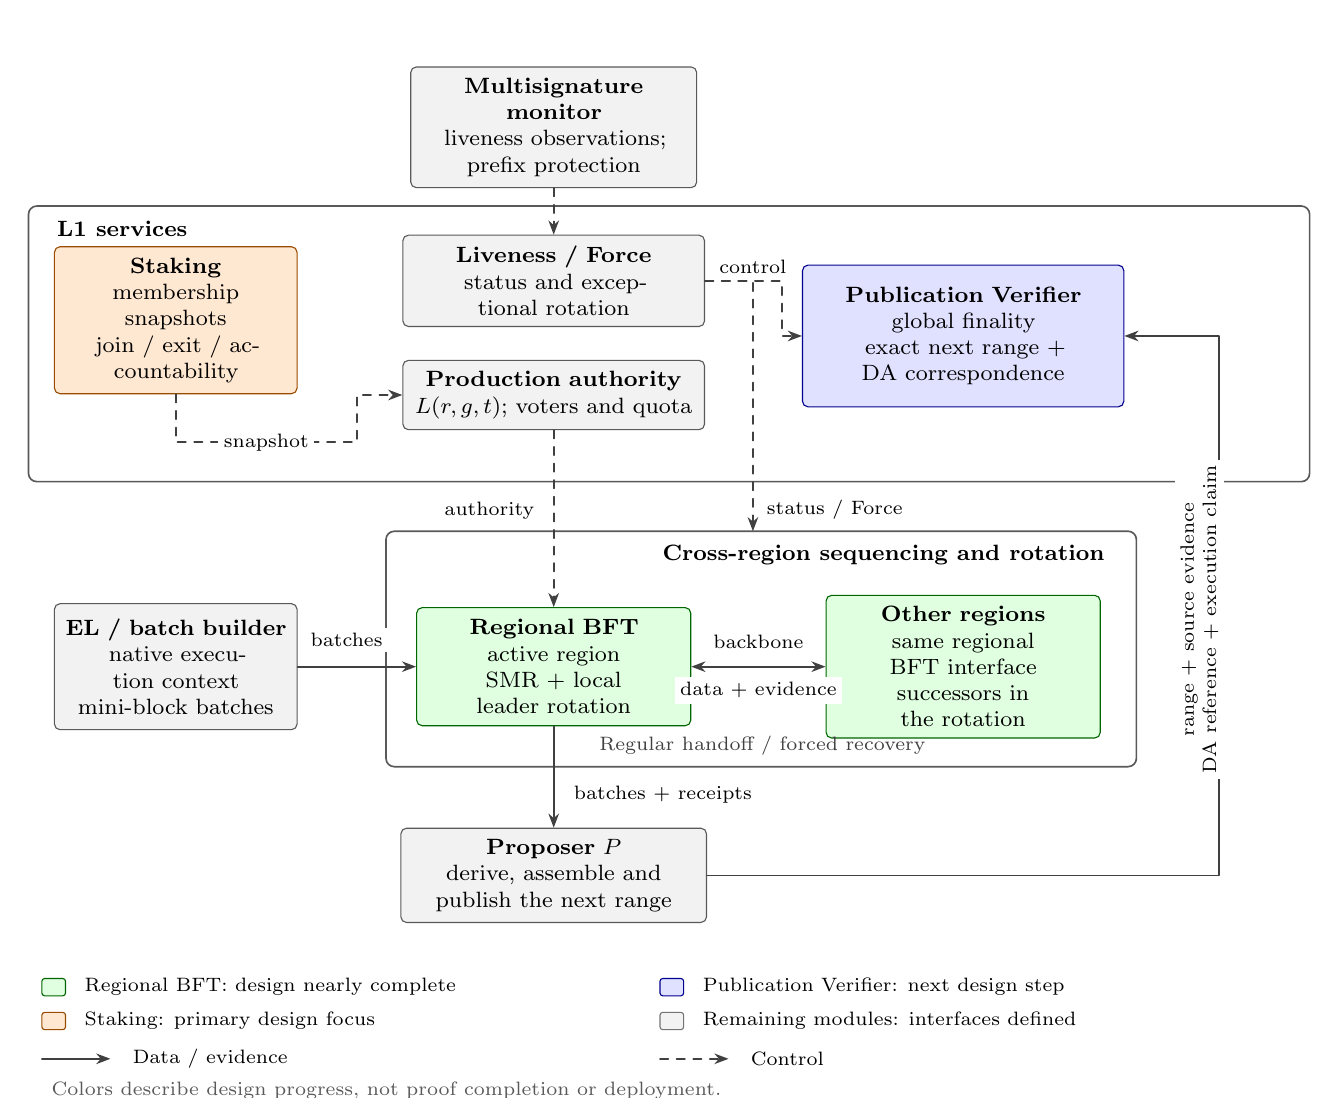
\begin{tikzpicture}[
  x=1cm,y=1cm,font=\footnotesize,line cap=round,line join=round,
  box/.style={draw=black!65,rounded corners=2pt,fill=gray!10,
    align=center,inner sep=4pt,minimum height=.86cm},
  ready/.style={box,fill=green!12,draw=green!40!black},
  next/.style={box,fill=blue!12,draw=blue!55!black},
  focus/.style={box,fill=orange!18,draw=orange!60!black},
  flow/.style={-{Stealth[length=1.8mm]},semithick,draw=black!75},
  ctl/.style={flow,dashed},
  lab/.style={fill=white,inner sep=2pt,align=center,font=\scriptsize},
  swatch/.style={draw=black!55,rounded corners=1pt,
    minimum width=.3cm,minimum height=.22cm,inner sep=0pt}
]
  % L1 and the service that is authorized to request exceptional control.
  \node[box,text width=3.35cm] (msig) at (6.85,11.05)
    {\textbf{Multisignature monitor}\\liveness observations; prefix protection};
  \draw[rounded corners=3pt,semithick,draw=black!65]
    (.18,6.55) rectangle (16.45,10.05);
  \node[anchor=west,font=\footnotesize\bfseries] at (.42,9.76)
    {L1 services};

  \node[focus,text width=2.8cm,minimum height=1.5cm] (stake) at (2.05,8.6)
    {\textbf{Staking}\\membership snapshots\\join / exit / accountability};
  \node[box,text width=3.55cm] (status) at (6.85,9.1)
    {\textbf{Liveness / Force}\\status and exceptional rotation};
  \node[box,text width=3.55cm] (authority) at (6.85,7.65)
    {\textbf{Production authority}\\$L(r,g,t)$; voters and quota};
  \node[next,text width=3.8cm,minimum height=1.8cm] (verify) at (12.05,8.4)
    {\textbf{Publication Verifier}\\global finality\\exact next range + DA correspondence};

  \draw[ctl] (msig.south) -- (status.north);
  \draw[ctl] (stake.south) -- (2.05,7.05) -- (4.35,7.05)
    -- (4.35,7.65) -- (authority.west);
  \node[lab] at (3.2,7.05) {snapshot};
  \draw[ctl] (status.east) -- (9.75,9.1) |- (verify.west);
  \node[lab,above] at (9.38,9.12) {control};

  % Native production feeds the regional service; the backbone joins regions.
  \node[box,text width=2.8cm,minimum height=1.6cm] (builder) at (2.05,4.2)
    {\textbf{EL / batch builder}\\native execution context\\mini-block batches};
  \draw[rounded corners=3pt,semithick,draw=black!65]
    (4.72,2.93) rectangle (14.25,5.92);
  \node[anchor=east,font=\footnotesize\bfseries] at (13.97,5.62)
    {Cross-region sequencing and rotation};
  \node[ready,text width=3.2cm,minimum height=1.5cm] (active) at (6.85,4.2)
    {\textbf{Regional BFT}\\active region\\SMR + local leader rotation};
  \node[ready,text width=3.2cm,minimum height=1.5cm] (other) at (12.05,4.2)
    {\textbf{Other regions}\\same regional BFT interface\\successors in the rotation};
  \node[font=\scriptsize,text=black!75] at (9.5,3.2)
    {Regular handoff / forced recovery};
  \draw[flow] (builder.east) -- (active.west);
  \node[lab] at (4.22,4.54) {batches};
  \draw[flow,{Stealth[length=1.8mm]}-{Stealth[length=1.8mm]}]
    (active.east) -- (other.west);
  \node[lab] at (9.45,4.52) {backbone};
  \node[lab] at (9.45,3.9) {data + evidence};

  \draw[ctl] (authority.south) -- (active.north);
  \node[lab,anchor=east] at (6.68,6.18) {authority};
  \draw[ctl] (status.east) -- (9.38,9.1) -- (9.38,5.92);
  \node[lab,anchor=west] at (9.48,6.2) {status / Force};

  % One publication module receives the range and its supporting evidence.
  \node[box,text width=3.6cm,minimum height=.96cm] (proposer) at (6.85,1.55)
    {\textbf{Proposer $P$}\\derive, assemble and publish the next range};
  \draw[flow] (active.south) -- (proposer.north);
  \node[lab,anchor=west] at (7.03,2.57) {batches + receipts};
  \draw[flow] (proposer.east) -- (15.3,1.55) -- (15.3,8.4)
    -- (verify.east);
  \node[lab,rotate=90] at (15.05,4.8)
    {range + source evidence\\DA reference + execution claim};

  % Compact legend: color is a work-plan marker, never a security claim.
  \node[swatch,fill=green!12,draw=green!40!black] at (.5,.13) {};
  \node[anchor=west,font=\scriptsize] at (.77,.13)
    {Regional BFT: design nearly complete};
  \node[swatch,fill=blue!12,draw=blue!55!black] at (8.35,.13) {};
  \node[anchor=west,font=\scriptsize] at (8.62,.13)
    {Publication Verifier: next design step};
  \node[swatch,fill=orange!18,draw=orange!60!black] at (.5,-.3) {};
  \node[anchor=west,font=\scriptsize] at (.77,-.3)
    {Staking: primary design focus};
  \node[swatch,fill=gray!10] at (8.35,-.3) {};
  \node[anchor=west,font=\scriptsize] at (8.62,-.3)
    {Remaining modules: interfaces defined};
  \draw[flow] (.35,-.78) -- (1.22,-.78);
  \node[anchor=west,font=\scriptsize] at (1.38,-.78) {Data / evidence};
  \draw[ctl] (8.2,-.78) -- (9.07,-.78);
  \node[anchor=west,font=\scriptsize] at (9.23,-.78) {Control};
  \node[anchor=west,font=\scriptsize,text=black!65] at (.35,-1.18)
    {Colors describe design progress, not proof completion or deployment.};
\end{tikzpicture}

\caption{The revised architecture, following the hand-drawn layout and
main v3's native diagram style. Staking supplies production authority;
regional BFT and the backbone deliver batches to $P$; one Publication
Verifier checks global finality, the next complete range and DA
correspondence. The monitor also receives complete backbone bundles,
and the verifier reads historical authorities;
these read paths are omitted to keep the main flows clear.}
\label{fig:architecture}
\end{figure}
% ARCH_V2_FIGURE_END

\section{Objects and module boundaries}\label{sec:objects}
One consensus DATA block $B_h$ contains one ordered batch $x_h$ of
mini-blocks. DATA height $h$, native mini-block number, and EVM block
number are separate indices. DRAIN is internal consensus bookkeeping and
has no application payload. A session is one region's production turn.
Its view is $(r,g,t)$: session index, recovery generation and leader term.

\begin{table}[H]\centering\small
\begin{tabularx}{\linewidth}{@{}p{.25\linewidth}Y@{}}
\toprule Shared object & Contract\\\midrule
Snapshot $S_e$ & Immutable regional members, keys and voting weights,
with protocol parameters recorded in authority.\\
$\api{AUTH}_{r,g}$ & L1 authority indexed by $(r,g)$.
$\api{AUTH}_{r,0}$ fixes the snapshot and quota; later generations
provide leader schedules only.\\
Session ID $\sigma_r$ & Hash of the boundary that opened the session.
It distinguishes branches even when they reuse the same index $r$.\\
Batch bundle $\mathcal B$ & DATA payloads, regional FINAL receipts,
ancestry, boundary witnesses and finalized L1 proofs, or resolvable
validated references to them.\\
Boundary witness $\mathcal W$ & REGULAR or FORCE transition, retained
anchor and evidence, successor and selection height.\\
Global checkpoint $G$ & A continuous DATA prefix commitment with height,
session IDs, historical authority and processed control context.\\
Publication checkpoint $C_{\rm pub}$ & The last accepted published prefix,
with DATA frontier $a\le h(G)$ and accepted execution state.\\
Publication claim $y$ & Previous accepted checkpoint, next DATA interval,
exact input commitment, DA commitment and execution-state transition.\\\bottomrule
\end{tabularx}
\caption{The objects shared by the modules. Certificate encodings and
storage layouts belong to their implementation documents.}
\end{table}

\textbf{Authority is indexed; evidence is branch-specific.}
Part II publishes $\api{AUTH}_{r,g}$ by numeric index because L1 need not
observe every regular boundary. A Force-created session reusing $r$
reads the same authority records for its selected region. Its new
$\sigma_r$ separates votes, locks, receipts and observation times.
The shorthand $L(r,g,t)$ means the leader selected from that authority
for the region assigned to the current session. Neither a Force nor
the current wall-clock epoch silently replaces the voting snapshot.

\textbf{Native compatibility.} Preserve the native mini-block encoding
and carry predecessor, BFT context and finalized L1 reference in an outer
DATA envelope. The envelope commits to the ordered native headers,
transaction bytes, receipts and boundaries. The pinned MegaETH baseline
and native-signing boundary are inherited from architecture v1:
\src{../megaeth_specs/specs/protocol/blocks.md}{blocks.md} and
\src{../megaeth_specs/specs/protocol/state-sync.md}{state-sync.md}
at \texttt{59797b45}. Native signing authority within an EVM block is
distinct from the current BFT leader. The EL adapter must provide a valid
execution and signing continuation at both regular and forced handoffs.

\section{Staking Service and authority: the main design work}\label{sec:staking}
\subsection{Participation and escrow}
\role Convert public stake-backed applications into immutable voting
snapshots, retain liability for earlier service, and release funds only
after the corresponding obligations end. Permissionless admission uses
public rules; it does not make a pending deposit an immediate voter.

\iface
\[
\begin{aligned}
 &\api{Join}(i,pk,\text{owner},b)\to o,\quad
   \api{Cancel}(o),\quad \api{RequestExit}(o),\\
 &\api{Report}(\text{evidence}),\qquad \api{Claim}(o).
\end{aligned}
\]
Here $o$ is a persistent stake-position identifier, $i$ its registered
region, $pk$ its signing key, and $b$ its bond. The initial profile follows
\src{../formalization/staking_rotation_module_v2.tex}{staking module v2}:
one collateral token, fixed region identifiers and whole-position joins
and exits. Delegation, partial withdrawal and region migration are
extensions. Key possession and withdrawal-owner authorization are checked
at the appropriate calls.

\begin{table}[H]\centering\small
\begin{tabularx}{\linewidth}{@{}p{.22\linewidth}Y@{}}
\toprule Lifecycle stage & Interface meaning\\\midrule
Pending join & Deposit is queued by finalized L1 order. No voting or
leader rights; cancellation is allowed before reservation.\\
Reserved & A frozen plan has selected the position. Its funds cannot be
refunded while activation is pending; the operator prepares to serve.\\
Assigned / active & A finalized authority uses its snapshot. The operator
serves whenever a valid boundary opens the corresponding session.\\
Exit queued & A request to stop receiving future duties. Existing
snapshot votes, participation and data duties remain in effect.\\
Retired / cooling & Retirement clearance establishes that no new valid
duties can arise and existing service obligations have ended. Required
data retention and evidence liability continue.\\
Claimable & Release residual funds after the liability window, retaining
amounts encumbered by timely unresolved claims.\\\bottomrule
\end{tabularx}
\caption{Permissionless entry and exit are a lifecycle, not immediate
edits to an active BFT committee.}
\end{table}

Queues and fixed cutoffs make selection reproducible. Separate inbound
and outbound stake/count budgets bound voluntary churn; canceling a
pending request cannot leave a permanent queue obstruction. Each permitted
whole position must fit its direction's budget. Mandatory removals after
penalties are accounted for separately. Under continued configuration
progress, eligible requests must receive service; an economic preference
for a regional stake floor cannot veto exit forever.

\subsection{Frozen plans and future authorities}\label{sec:authority}
\role Publish a reproducible mapping from stake snapshots to the
authorities consumed by Part II. Authority establishes eligibility;
the REGULAR/FORCE boundary and Ready establish actual session entry.

\iface
\[
\begin{aligned}
 &\api{Prepare}(e)\to\mathit{Plan}_e,\qquad
   \api{Activate}(\mathit{Plan}_e,\mathcal I_e),\\
 &\api{ReadSnapshot}(e)\to S_e,\qquad
   \api{ReadAuthority}(r,g)\to\api{AUTH}_{r,g}.
\end{aligned}
\]
$\mathcal I_e$ is a finite set or range of future, as-yet-unassigned
session indices. Assigning a range is an architectural option for
amortizing L1 updates, not an extra transaction at each handoff.
\api{Prepare} fixes the selected joins/exits and balances at the public
cutoff. If randomness is used, freeze the plan before obtaining the
prescribed random input and forbid discretionary retries.

\api{Activate} accepts only a frozen, publicly verifiable plan and
establishes an immutable mapping $e(r)$ for the assigned indices, so
the relevant snapshot in $\api{AUTH}_{r,0}$ is $S_{e(r)}$.
An already assigned index cannot be rebound. The snapshot includes
regional members, keys, weights, $F_i$, $\Delta_i$ and $K$; the authority
also fixes $\TB_r$. For $g>0$, only the new leader schedule is consumed.
The admissible index range and activation condition follow public policy;
the relayer cannot choose them to favor a particular plan or skip queues.
Later finalized schedules can exclude exposed equivocators, while votes
remain measured against the original snapshot. Already finalized
schedules cannot be retroactively rewritten.

The authority service must give members timely access to the rules for
future indices and recovery generations, and must leave actual future
service opportunities for new snapshots. An unbounded advance allocation
of indices to an old snapshot would defeat admission and exit. If a needed
authority is not finalized, Part II waits. A zero-member region must not
be selected as live under the authority/control combination. Part II's
fixed cyclic region order and \api{NextLive} rule are retained; this
architecture does not import the staking draft's per-epoch region shuffle
or same-region renewal.

\subsection{Retirement clearance and withdrawal}\label{sec:retirement}
\role Connect removal from future stake plans to the end of actual
consensus duties. This is the central unresolved staking interface.
\api{Retired}(o,\text{clearance}) is a lifecycle event produced only after
the service can establish:
\begin{enumerate}
\item future authority assignment will not create new duties for $o$;
\item consensus and signing duties from already assigned indices are
discharged, including
sessions that a valid Force could still open using an old index; and
\item already opened regional engines have reached an allowed stopping
condition, with required history retained or transferred.
\end{enumerate}
The clearance must bind the relevant historical authorities and session
IDs. A new epoch, a region-off status or a Force activation alone does
not establish it. Part II leaves discarded engines running until their
Completion condition; it has no general early-stop rule. Therefore this
index does not assert a bounded withdrawal time. The staking design must
provide retirement clearance or explicitly retain that dependency.

After clearance, the liability/retention policy sets the release horizon.
Timely accepted unresolved claims retain the affected escrow until
adjudication. Slashing reduces the remaining bond, never the historical
quorum denominator; the same funds cannot be recovered independently
once per old epoch. Equivocation evidence binds the old position,
authority and session ID. Timeout BLAME or a health report is not by
itself slashable equivocation. Historical certificate acceptance and
key-compromise assumptions must match the liability/checkpoint policy.

These interfaces reuse staking v2's queues, reservations and escrow
semantics. They replace its \api{Close}/\api{Advance} coupling: ordinary
Part II handoffs remain off L1, and Force does not close the old regional
engine. Churn and staking alone do not establish $F_i<W_i/2$ in every
serving region.

\section{Multisignature monitor and Liveness/Force Control}\label{sec:force}
\subsection{Off-chain monitoring}
\role The multisignature service diagnoses regional health, keeps Part
II's protected prefix, and submits control updates. Treat it initially
as one honest, coordinated service. Its internal membership mechanism
is outside this architecture.

\iface
\[
 \api{ObserveBundle}(\mathcal B),\quad
 \api{ReportHealth}(i,\text{observations}),\quad
 \api{SubmitControl}(U).
\]
Record first complete validation at $\mu(B)$. At
$\mu(B)+T_{\rm msig}$, if $B$ remains on the current branch, protect the
next continuous prefix unless $B$ lies in the outstanding Force's deletion
scope. Actual Force submission rechecks that its deletion scope is disjoint
from the protected prefix. A suitable receipt-backed anchor is enough;
it need not be the highest regional commitment. Its data and evidence
must remain available outside the failed region. Health diagnosis
affects liveness policy; it does not certify data or execution.

\subsection{L1 control interface}
\role Authenticate and order status/Force records, making their
finalization and activation visible to rotation and the Publication Verifier.

\iface
\[
 \api{Status}(\chi,\lambda_a),\quad
 \api{Force}(\sigma_r,r,h_*,\chi,\lambda_a),\quad
 \api{ReadControl}(\lambda).
\]
A Force also binds the chain. $h_*$ is the retained DATA height on the
target session, and its map marks that region off. An update included
at $\lambda_p$ must satisfy $\lambda_a\ge\lambda_p+N$, with increasing
activation heights. The monitor submits an update only after all earlier
updates are finalized. One fixed Force can be outstanding through
activation; each session ID can be targeted at most once.

\begin{center}\small
\begin{tabularx}{\linewidth}{@{}p{.21\linewidth}Y@{}}
\toprule Stage & Effect exposed to other modules\\\midrule
Submitted & Monitor records the fixed deletion scope $\Del(F)$ at
actual submission; collected signatures alone do not start this stage.\\
L1 finalized & The verifier and other observers block global promotion of
$\Del(F)$ immediately, even before activation.\\
L1 activated & Finalization of block $\lambda_a$ changes eligibility
and replaces the external branch; successor bootstrap becomes possible.\\\bottomrule
\end{tabularx}
\end{center}
The deletion scope includes the target suffix above $h_*$ and every
descendant of its replaced regular boundary, even when $h_*=H_r$.
Passive updates do not interrupt the current session. Until activation,
regional production and regular handoffs can continue. None of these
control stages rewrites an old regional log or its voting weights.

\section{EL, regional BFT and the backbone}\label{sec:sequencing}
\subsection{EL and batch builder}
\role Construct a valid ordered batch and its native execution context.
Regional BFT orders this application input; the builder's packing policy
is a separate concern.

\iface
\[
 \api{Build}(\text{parent context},\text{requests})\to x,\qquad
 \api{ValidBatch}(x;\text{parent context}).
\]
Validation binds exact bytes, order, multiplicity, mini-block boundaries,
native positions and permitted block context. For full native mini-blocks,
receipts and gas fields must be consistent with execution. Publication
progress requires a publishable execution continuation, established by
execution, sound evidence or an explicit application-validity assumption.
Rejecting an invalid globally committed batch only at publication time
can block the entire publication stream, since $P$ cannot skip it.

The native adapter owns EVM-boundary assembly and signing-key continuity
when BFT leaders or regions change. An empty DATA payload is allowed and
consumes quota without creating a native EVM block. Requests remain pending
until global inclusion, and discarded regional suffixes return their
requests to consideration under Part II's admission and queue rules.

\subsection{Regional BFT and cross-region composition}
\role Provide fixed-snapshot SMR, regular in-region leader rotation,
failure recovery and regional commit evidence. The cross-region handler
then composes these engines through certified boundaries. The green
Regional BFT boxes in Figure~\ref{fig:architecture} denote the same
nearly completed engine instantiated in different regions.

\iface
\[
\begin{aligned}
 &\api{Open}(\sigma_r,\mathcal W,\api{AUTH}_{r,0}),\quad
   \api{Propose}(x),\quad \api{RegionalOutput}(B,\pi_R),\\
 &\api{Boundary}(\mathcal W),\qquad
   \api{BranchChanged}(G_{\rm retained},\mathcal W).
\end{aligned}
\]
A receipt $\pi_R$ is a valid FINAL receipt, or same-session covering
receipt with verified ancestry. It requires weight $>F_i$ under the
fixed snapshot, where $F_i<W_i/2$. It establishes regional commitment;
the external verifier separately checks that rotation assigned the block
to this region and session. A proposal QC does not replace the receipt.

Normal leader rotation uses a terminal QC below the session endpoint
$H_r=h(A_{r,0,0})+\TB_r$ and preserves commit timers. Recovery changes
generation and waits for its authority, preserving the snapshot and quota.
At the endpoint, recovery-only DRAIN can complete the terminal DATA
commitment. Part II's Completion step stops a replica's production,
voting and unfinished timers once it holds the terminal regional receipt;
the replica continues serving data.

A regular boundary inherits $T_r$ and its receipt; a forced boundary
inherits the retained anchor of an activated Force. \api{NextLive}
chooses the first other live region at Part II's deterministic selection
height. Each successor member enters at its own Ready event after
validating the full witness, data and authority. With no other live
region, rotation waits. Normal handoff waits for neither publication
verification nor a new L1 transaction. Force changes the external branch,
not the old engine's local commitment state.

\subsection{Backbone and data retention}
\role Carry complete batches, receipts and witnesses between regions,
the monitor and $P$, and make retained anchors recoverable.

\iface
\[
 \api{Publish}(\mathcal B),\qquad \api{Fetch}(\text{range or object}),
 \qquad \api{RelayMonitor}(\mathcal B).
\]
Ordinary backbone delivery is eventual. The monitor path additionally
meets $T_{\rm mon}$, including missing-data retrieval and full validation.
These are separate service guarantees. Native state-sync streams may be
reused alongside the BFT evidence path. Transport does not choose a
leader, grant finality or replace rollup DA. Data duties survive until
the applicable recovery, publication and retirement obligations end.

\section{Publication Verifier: finality and DA publication}\label{sec:publication}
\role Accept a proposer's DA publication only when it contains exactly
the next complete range of globally final mini-block batches. This single
L1 module combines Part II's global-finality tracking with range and DA
correspondence checks. Global tracking is its internal state-maintenance
logic; it does not add a global voting round or change regional BFT.

\subsection{State and interface}
The verifier keeps two distinct frontiers:
\begin{itemize}
\item $G$: the globally final DATA prefix, with its historical authority
and session provenance;
\item $C_{\rm pub}$: the prefix whose publication has been accepted,
with DATA frontier $a\le h(G)$ and accepted execution state $z_{\rm pub}$.
\end{itemize}
Global finality can advance before $P$ publishes the data. The verifier
also keeps a verified provisional branch, its processed finalized-control
context, and first observation records keyed by $(\sigma_r,\Hash(B))$.
Its core publication interface and supporting calls are:
\[
 \api{VerifyAndAccept}(y,\pi)\to C_{\rm next},
\]
\[
 \api{Observe}(\mathcal B),\qquad
 \api{Frontiers}()\to(G,C_{\rm pub}).
\]
Here $y$ is the publication claim defined below, and $\pi$ contains its
source/range, DA and execution evidence. Any relayer, including $P$, may
supply complete evidence. Invalid or incomplete input cannot start a
finality timer. Internally, \api{Advance} maintains $G$ and
\api{VerifyRange} checks exact membership of a whole interval in that
prefix. A height comparison or a proof of a few leaves is insufficient.
\api{VerifyAndAccept} advances global state as the evidence and waiting
rules permit, then applies all publication acceptance checks.

\api{Observe} verifies regional finality: historical authority, branch
assignment, receipts, payloads and ancestry. It records $s_{\rm V}(B)$
only when complete validation and the bounded relay to the monitor are
established. Registration is idempotent. New receipt encodings cannot
reset a timer; another session ID at the same height is a different
candidate. Newly registered blocks in a range may use a later common
start as a conservative optimization; previously observed or retained
blocks keep their original starts.

\subsection{Internal global-finality tracking}\label{sec:tracker}
Before \api{Advance}, refresh the finalized L1 control view and apply
due Force processing. Starting immediately after $G$, the next DATA
block $B$ may be promoted when the following conditions hold:
\[
\begin{aligned}
 &\RF(B;\text{current finalized control})=1,\\
 &\text{all DATA predecessors of }B\text{ are already in }G,\\
 &\api{Elapsed}(s_{\rm V}(B),\text{now})\ge\Twait,
   \qquad \Twait=T_{\rm mon}+T_{\rm msig}+T_{\rm L1},\\
 &B\notin\Del(F)\quad\text{for every applicable finalized Force }F.
\end{aligned}
\]
Stop at the first block that fails. Finalized Force processing precedes
promotion at an equal deadline. A finalized but inactive Force already
blocks its deletion scope. Activation replaces only the provisional
branch; the global checkpoint never rolls back. A purported Force that
would remove $G$ is a control-service violation, not a rollback command.

\textbf{L1 implementation contract.} The on-chain realization must
provide three facts used by this same rule:
\begin{enumerate}
\item complete registered data are relayed so the monitor validates
them within $T_{\rm mon}$ of the recorded start;
\item \api{Elapsed} is a conservative measure of time since that
validation-and-relay event on Part II's clock; and
\item the control view used at promotion includes every finalized Force
available at that decision time. If it is unavailable, promotion waits.
\end{enumerate}
An L1 registration/event plus a monitoring adapter is the intended
integration surface. Its exact finalization and time mapping must be
specified for the chosen L1; neither a caller-supplied old time nor the
DATA block's old L1 reference supplies these facts. Part II does not
equate an L1 block timestamp with the time it became finalized. These
are implementation obligations of the verifier, not another certificate
or a multisignature acknowledgement added to the regional protocol.

Off-chain observers may continue using Part II directly. Observation and
publication calls may cover ranges; regional production and normal
handoffs do not depend on those calls. Consumers use the verifier state
confirmed under L1 finality, not a tentative transaction receipt.
Under Part II's regional, monitor and timing
assumptions, the verifier maintains an irreversible global prefix.

\subsection{Publication acceptance}
Let $a$ be the accepted publication frontier. A claim is
\[
 y=(C_{\rm prev},[a+1,b],C_{\rm in},C_{\rm DA},z_{\rm pre},z_{\rm post}).
\]
The structured $C_{\rm in}$ binds native headers, transaction order and
multiplicity, mini-block boundaries and execution context. The verifier
accepts $y$ only if:
\begin{enumerate}
\item $C_{\rm prev}=C_{\rm pub}$ and $z_{\rm pre}=z_{\rm pub}$; the
range begins immediately after the last accepted position;
\item the internal \api{VerifyRange} check binds $C_{\rm in}$ to exactly
$[a+1,b]$ in $G$, with no omitted, inserted, reordered or replayed positions;
\item decoding the data committed by $C_{\rm DA}$ gives that same
structured input, and the chosen DA mechanism's availability/retention
predicate holds; and
\item the execution-verification interface confirms that this input
transforms $z_{\rm pre}$ into $z_{\rm post}$, with recomputed receipts,
gas and native block assembly matching its commitments.
\end{enumerate}
Checking that every submitted mini-block is individually global is not
enough: the range must be the complete next interval, and the DA data
must match it. A DA certificate supplies availability evidence under its
own service contract; it does not replace the global-finality or
correspondence checks. The accepted update advances $C_{\rm pub}$ to
$C_{\rm next}$ at height $b$ and sets $z_{\rm pub}=z_{\rm post}$.
It does not make an unconfirmed block global.

Native system transactions are committed or deterministically derived by
the agreed adapter; $P$ cannot insert discretionary user transactions.
The publication endpoint must support the native execution checkpoint,
or bind an explicitly supported partial-EVM continuation. Execution
correctness remains a separate verification responsibility whose result
this module consumes. It may use direct checks, a validity proof or a
sound dispute procedure. A pending or disputed claim does not advance
the accepted publication frontier until verification completes.

\section{Proposer $P$}\label{sec:proposer}
\role Fetch certified batches, prepare native execution and DA data,
and submit the next complete publication interval to the Publication
Verifier. $P$ may work on regional output speculatively; final acceptance
requires the globally final range and all publication checks above.

\iface $P$ submits $(y,\pi)$ through \api{VerifyAndAccept} and may use
\api{Observe} to supply supporting regional evidence. It has no privileged
power to declare input global. After a Force, retained backlog from the
old region still precedes new input. Proposer replacement resumes from
$C_{\rm pub}$, which may lag both production and global finality.

Faithful acceptance is a safety property even for Byzantine $P$.
Eventual publication also needs an available proposer or replacement
path, native signing/execution availability and DA service. The verifier
does not make an absent proposer publish.

\section{Module index and next design steps}\label{sec:index}
\begin{table}[H]\centering\small
\begin{tabularx}{\linewidth}{@{}p{.23\linewidth}Y Y@{}}
\toprule Module & Primary design source & Next deliverable\\\midrule
Regional BFT & Part I; Part II regional definitions and protocols
& Finish the current engine review and its stated conditional analyses.\\
Publication Verifier & Part II finality and observer rules; main v3
publication relation; \cref{sec:publication}
& Implement global tracking and exact-range/DA checks behind
VerifyAndAccept, with the clock/relay and execution interfaces.\\
Staking / authority & Staking v2 participation and escrow;
\cref{sec:staking,sec:authority,sec:retirement}
& Freeze/activate future authorities and establish retirement clearance
and withdrawal liability.\\
Monitor / Force & Part II model and Force handler; \cref{sec:force}
& Control-record encoding and monitoring/submission service.\\
EL / backbone & Architecture v1 native/transport contracts;
\cref{sec:sequencing}
& Native execution/signing continuation, complete-bundle retrieval
and retention.\\
Proposer & Main v3 publication relation; \cref{sec:proposer}
& Assemble the next complete range, publish its DA data and supply
the evidence required by the verifier.\\\bottomrule
\end{tabularx}
\caption{Index to the submodule designs. The priority colors in
Figure~\ref{fig:architecture} separate the immediate publication-verifier task from
the larger staking lifecycle design.}
\end{table}

The integration order is: retain the current regional protocol interface;
realize its global rule and faithful DA publication in the Publication
Verifier; then complete the staking
lifecycle around index-keyed authority. The staking work must account
for Force reuse and unfinished old engines. Moving global verification
on chain does not itself provide retirement clearance or change the
regional fault assumption.

Global-finality tracking and DA publication verification form one L1
module. It keeps the global prefix and the accepted publication frontier
as separate internal states and exposes \api{VerifyAndAccept} to $P$. The
authority interface follows Part II's $(r,g)$ keys and immutable
$\api{AUTH}_{r,0}$ snapshots. The original goals and the separate roles
of regional consensus, liveness management, native execution and faithful
publication remain the same.
\end{document}
